\subsection{Instalar Bacula Client en Windows}


Primero descargamos Bacula. Para ello, visitamos el sitio web oficial y navegamos a la sección de descargas para Windows.

\begin{figure}[H]
    \centering
    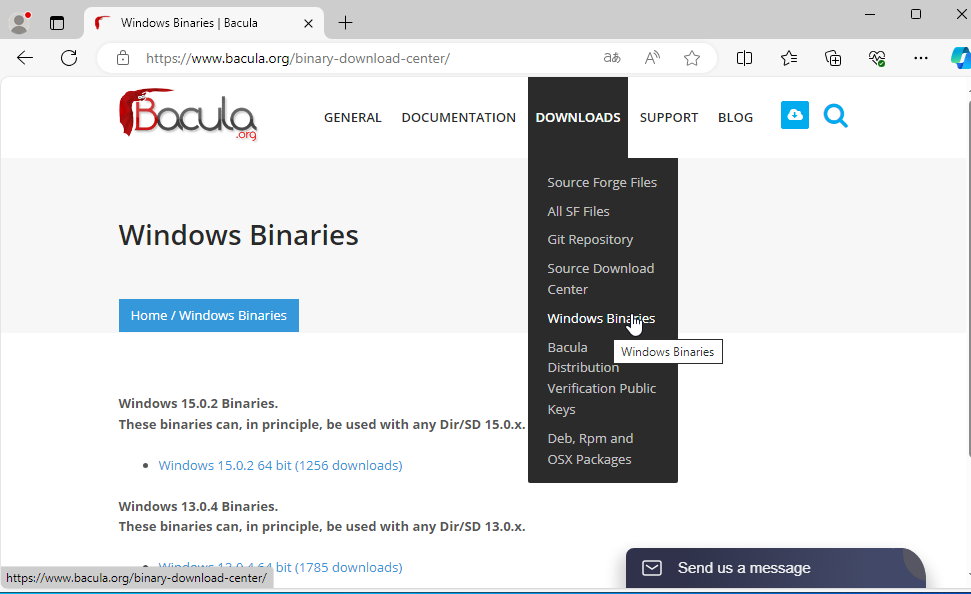
\includegraphics[width=0.5\linewidth]{instalacionBacula/winbinaries.png}
    \caption{Página de descargas de Bacula para Windows.}
\end{figure}

Descargamos la última versión disponible.

\begin{figure}[H]
    \centering
    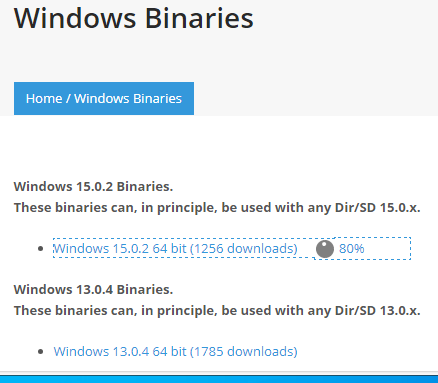
\includegraphics[width=0.5\linewidth]{instalacionBacula/downloadwinbinaries.png}
    \caption{Descarga de la última versión de Bacula para Windows.}
\end{figure}

Iniciamos el instalador que hemos descargado.

\begin{figure}[H]
    \centering
    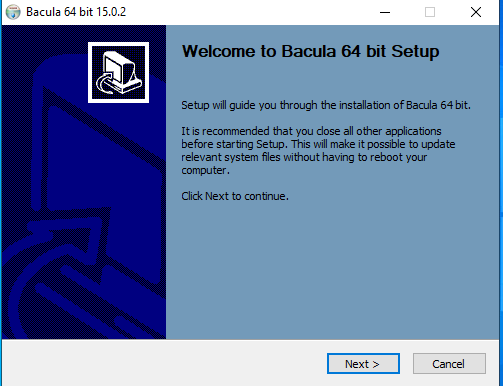
\includegraphics[width=0.5\linewidth]{instalacionBacula/instalador.png}
    \caption{Instalador de Bacula para Windows.}
\end{figure}

Aceptamos el acuerdo de licencia para continuar con la instalación.

\begin{figure}[H]
    \centering
    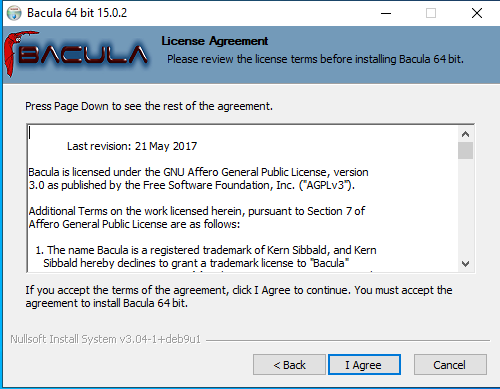
\includegraphics[width=0.5\linewidth]{instalacionBacula/lecencia.png}
    \caption{Acuerdo de licencia de Bacula.}
\end{figure}

Elegimos el tipo de instalación. En este caso, optamos por la instalación personalizada (Custom) para configurar específicamente los componentes del cliente.

\begin{figure}[H]
    \centering
    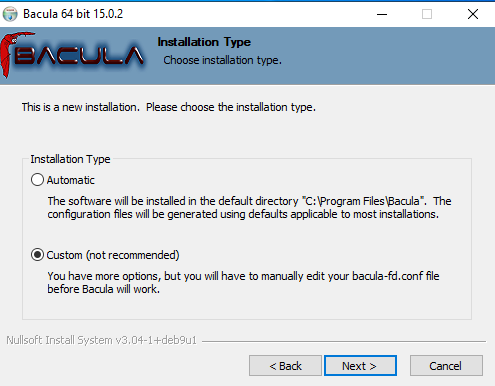
\includegraphics[width=0.5\linewidth]{instalacionBacula/custom.png}
    \caption{Selección del tipo de instalación en Bacula.}
\end{figure}

Seleccionamos las características específicas para instalar solo el cliente de Bacula.

\begin{figure}[H]
    \centering
    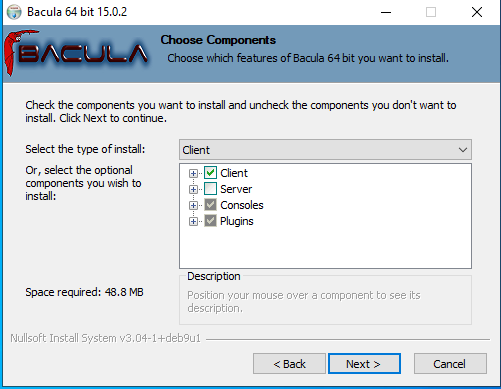
\includegraphics[width=0.5\linewidth]{instalacionBacula/clientecaracteristicas.png}
    \caption{Selección de componentes del cliente Bacula durante la instalación.}
\end{figure}

\textbf{Nota:} Es importante asegurarse de que solo se seleccionen los componentes necesarios para la funcionalidad del cliente, para evitar instalaciones innecesarias de otros componentes del servidor.


Elegimos la ruta de instalación.

\begin{figure}[H]
    \centering
    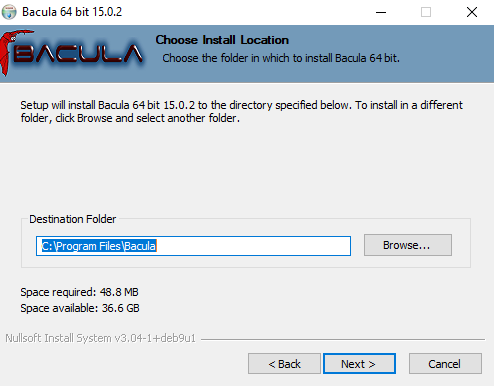
\includegraphics[width=0.5\linewidth]{instalacionBacula/rutawindebacula.png}
    \caption{Elección de la ruta de instalación de Bacula.}
\end{figure}

Aplicamos la configuración del cliente, puerto, y máximo de trabajos simultáneos.

\begin{figure}[H]
    \centering
    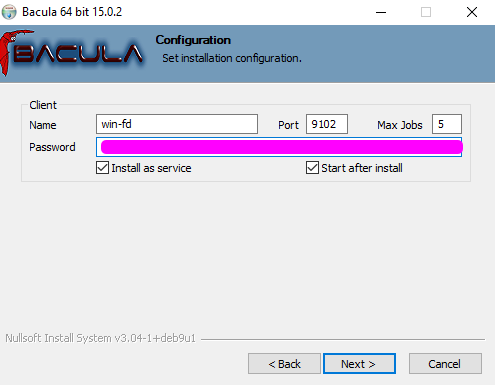
\includegraphics[width=0.5\linewidth]{instalacionBacula/configwinbaCULA.png}
    \caption{Configuración del cliente Bacula en Windows.}
\end{figure}

También configuramos la información del Director.

\begin{figure}[H]
    \centering
    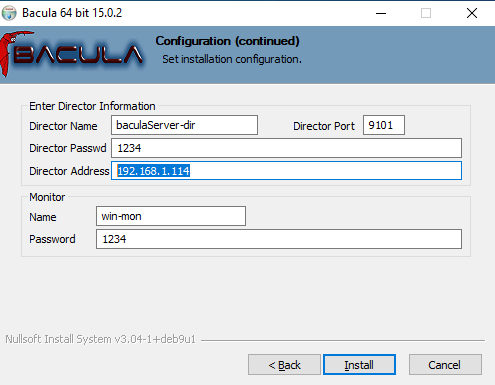
\includegraphics[width=0.5\linewidth]{instalacionBacula/config2winbacula.png}
    \caption{Configuración del Director en Bacula.}
\end{figure}

Instalamos y esperamos a que termine.

\begin{figure}[H]
    \centering
    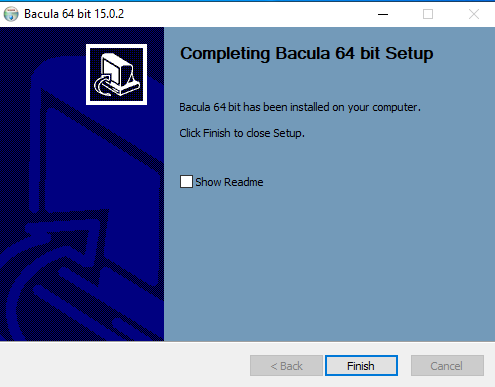
\includegraphics[width=0.5\linewidth]{instalacionBacula/teminadoInstalarBaculawin.png}
    \caption{Finalización de la instalación de Bacula en Windows.}
\end{figure}

Ahora en el firewall de Windows, añadimos Bacula al firewall.

\begin{figure}[H]
    \centering
    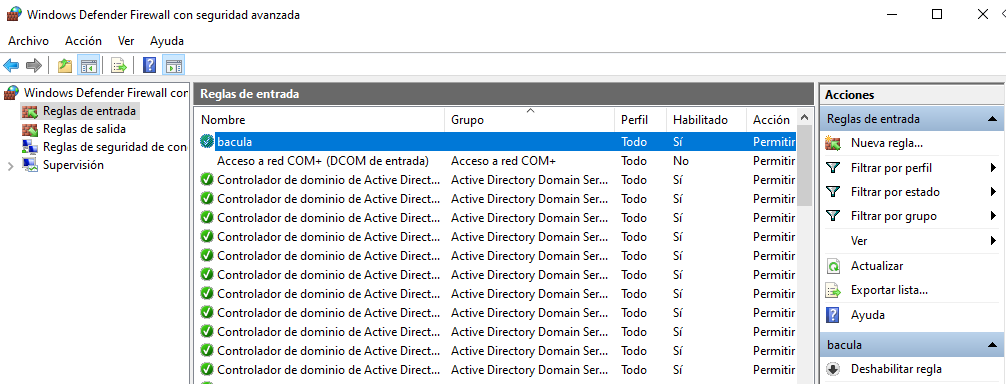
\includegraphics[width=0.5\linewidth]{instalacionBacula/firewallwindows.png}
    \caption{Configuración del Firewall para Bacula.}
\end{figure}

Permitimos que el servicio interactúe con el escritorio en el panel de servicios de Windows.

\begin{figure}[H]
    \centering
    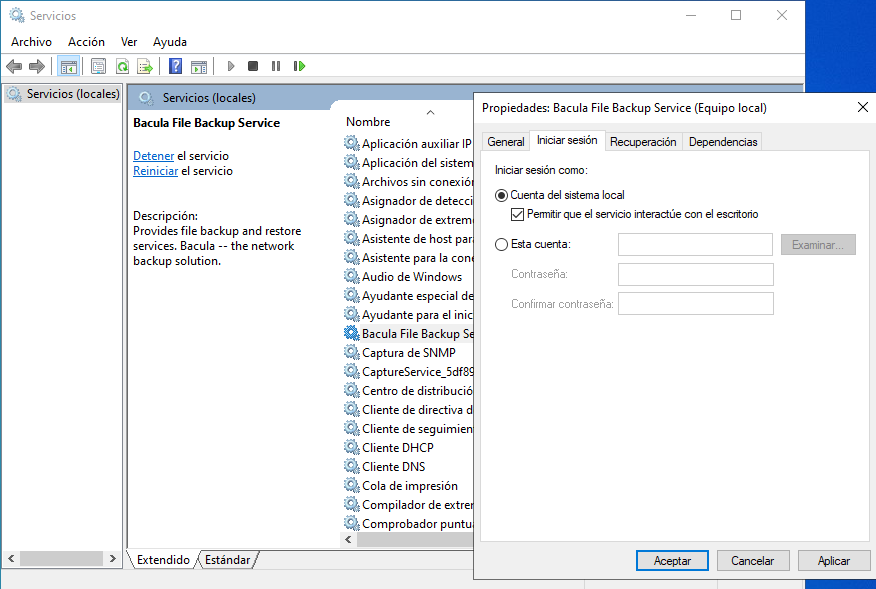
\includegraphics[width=0.5\linewidth]{instalacionBacula/permitirservicio.png}
    \caption{Permitir la interacción del servicio de Bacula con el escritorio.}
\end{figure}
